%
%Не забыть:
%--------------------------------------
%Вставить колонтитулы, поменять название на титульнике



%--------------------------------------

\documentclass[a4paper, 12pt]{article} 

%--------------------------------------
%Russian-specific packages
%--------------------------------------
%\usepackage[warn]{mathtext}
\usepackage[T2A]{fontenc}
\usepackage[utf8]{inputenc}
\usepackage[english,russian]{babel}
\usepackage[intlimits]{amsmath}
\usepackage{esint}
%--------------------------------------
%Hyphenation rules
%--------------------------------------
\usepackage{hyphenat}
\hyphenation{ма-те-ма-ти-ка вос-ста-нав-ли-вать}
%--------------------------------------
%Packages
%--------------------------------------
\usepackage{amsmath}
\usepackage{amssymb}
\usepackage{amsfonts}
\usepackage{amsthm}
\usepackage{latexsym}
\usepackage{mathtools}
\usepackage{etoolbox}%Булевые операторы
\usepackage{extsizes}%Выставление произвольного шрифта в \documentclass
\usepackage{geometry}%Разметка листа
\usepackage{indentfirst}
\usepackage{wrapfig}%Создание обтекаемых текстом объектов
\usepackage{fancyhdr}%Создание колонтитулов
\usepackage{setspace}%Настройка интерлиньяжа
\usepackage{lastpage}%Вывод номера последней страницы в документе, \lastpage
\usepackage{soul}%Изменение параметров начертания
\usepackage{hyperref}%Две строчки с настройкой гиперссылок внутри получаеммого
\usepackage[usenames,dvipsnames,svgnames,table,rgb]{xcolor}% pdf-документа
\usepackage{multicol}%Позволяет писать текст в несколько колонок
\usepackage{cite}%Работа с библиографией
\usepackage{subfigure}% Человеческая вставка нескольких картинок
\usepackage{tikz}%Рисование рисунков
\usepackage{float}% Возможность ставить H в положениях картинки
% Для картинок Моти
\usepackage{misccorr}
\usepackage{lscape}
\usepackage{cmap}

% Для Х И М И И

\usepackage{mhchem}



\usepackage{graphicx,xcolor}
\graphicspath{{Pictures/}}
\DeclareGraphicsExtensions{.pdf,.png,.jpg}

%----------------------------------------
%Список окружений
%----------------------------------------
\newenvironment {theor}[2]
{\smallskip \par \textbf{#1.} \textit{#2}  \par $\blacktriangleleft$}
{\flushright{$\blacktriangleright$} \medskip \par} %лемма/теорема с доказательством
\newenvironment {proofn}
{\par $\blacktriangleleft$}
{$\blacktriangleright$ \par} %доказательство
%----------------------------------------
%Список команд
%----------------------------------------
\newcommand{\grad}
{\mathop{\mathrm{grad}}\nolimits\,} %градиент

\newcommand{\diver}
{\mathop{\mathrm{div}}\nolimits\,} %дивергенция

\newcommand{\rot}
{\ensuremath{\mathrm{rot}}\,}

\newcommand{\Def}[1]
{\underline{\textbf{#1}}} %определение

\newcommand{\RN}[1]
{\MakeUppercase{\romannumeral #1}} %римские цифры

\newcommand {\theornp}[2]
{\textbf{#1.} \textit{ #2} \par} %Написание леммы/теоремы без доказательства

\newcommand{\qrq}
{\ensuremath{\quad \Rightarrow \quad}} %Человеческий знак следствия

\newcommand{\qlrq}
{\ensuremath{\quad \Leftrightarrow \quad}} %Человеческий знак равносильности

\renewcommand{\phi}{\varphi} %Нормальный знак фи

\newcommand{\me}
{\ensuremath{\mathbb{E}}}

\newcommand{\md}
{\ensuremath{\mathbb{D}}}



%\renewcommand{\vec}{\overline}




%----------------------------------------
%Разметка листа
%----------------------------------------
\geometry{top = 3cm}
\geometry{bottom = 2cm}
\geometry{left = 1.5cm}
\geometry{right = 1.5cm}
%----------------------------------------
%Колонтитулы
%----------------------------------------
\pagestyle{fancy}%Создание колонтитулов
\fancyhead{}
%\fancyfoot{}
\fancyhead[R]{\textsc{Гидролиз солей. Гидрокомплексы металлов и их свойства}}%Вставить колонтитул сюда
%----------------------------------------
%Интерлиньяж (расстояния между строчками)
%----------------------------------------
%\onehalfspacing -- интерлиньяж 1.5
%\doublespacing -- интерлиньяж 2
%----------------------------------------
%Настройка гиперссылок
%----------------------------------------
\hypersetup{				% Гиперссылки
	unicode=true,           % русские буквы в раздела PDF
	pdftitle={Заголовок},   % Заголовок
	pdfauthor={Автор},      % Автор
	pdfsubject={Тема},      % Тема
	pdfcreator={Создатель}, % Создатель
	pdfproducer={Производитель}, % Производитель
	pdfkeywords={keyword1} {key2} {key3}, % Ключевые слова
	colorlinks=true,       	% false: ссылки в рамках; true: цветные ссылки
	linkcolor=blue,          % внутренние ссылки
	citecolor=blue,        % на библиографию
	filecolor=magenta,      % на файлы
	urlcolor=cyan           % на URL
}
%----------------------------------------
%Работа с библиографией (как бич)
%----------------------------------------
\renewcommand{\refname}{Список литературы}%Изменение названия списка литературы для article
%\renewcommand{\bibname}{Список литературы}%Изменение названия списка литературы для book и report
%----------------------------------------
\begin{document}
	\begin{titlepage}
		\begin{center}
			$$$$
			$$$$
			$$$$
			$$$$
			{\Large{НАЦИОНАЛЬНЫЙ ИССЛЕДОВАТЕЛЬСКИЙ УНИВЕРСИТЕТ}}\\
			\vspace{0.1cm}
			{\Large{ВЫСШАЯ ШКОЛА ЭКОНОМИКИ}}\\
			\vspace{0.25cm}
			{\large{Факультет физики}}\\
			\vspace{5.5cm}
			{\Huge\textbf{{Лабораторная работа}}}\\%Общее название
			\vspace{1cm}
			{\LARGE{<<Гидролиз солей. Гидрокомплексы металлов и их свойства>>}}\\%Точное название
			\vspace{2cm}
			{Работу выполнил студент 2 курса}\\
			{Никитин Илья Сергеевич}
			\vfill
			
\includegraphics[width = 0.2\textwidth]{HSElogo}\\
			\vfill
			Москва\\
			10 апреля 2021
		\end{center}
	\end{titlepage}

\tableofcontents

\newpage
\section{Опыт 1.1: Кислотно-основное титрование}
\subsection{Метод выполнения работы}

В ходе выполнение работы предполагалось провести титрование раствора соляной кислоты HCl раствором гидроксида натрия NaOH с целью определения реальной концентрации раствора NaOH.

Для этого сперва была приготовлена навеска гидроксида натрия для получение 100 мл раствора предполагаемой концентрацией 0.1M. Для расчета массы воспользуемся определением молярной концентрации:

\begin{equation}
C_m = \frac{m}{M V} \qrq m = C_m M V
\label{eq:NaOH_mass}
\end{equation}

Здесь $m$ --- масса растворенного вещества, $M$ --- его молярная масса, $V$ --- объем. С учетом того, что 0.1M означает 0.1 моль/л, примем следующие значения:

\begin{itemize}
	\item $M = 40$ г/моль 
	
	\item $V = 0.1$ л (необходимый объем раствора)
	
	\item $C_m = 0.1 \text{M}$
\end{itemize}

Таким образом, по формуле \ref{eq:NaOH_mass} получаем, что необходимая масса NaOH составляет $m_t = 0.4$~г. Данная масса была отмерена с помощью аналитических весов.

Раствор NaOH был получен следующим образом: сперва в мерную колбу на 100 мл была помещена навеска NaOH, после чего к ней была добавлен небольшой объем воды (порядка 40 мл). Затем, после тщательного перемешивания, была долита оставшаяся вода до отметки 100 мл.

Небольшим объемом получившегося раствора щелочи была промыта бюретка, после чего она была заполнена до нулевой отметки этим же раствором.

\begin{center}
	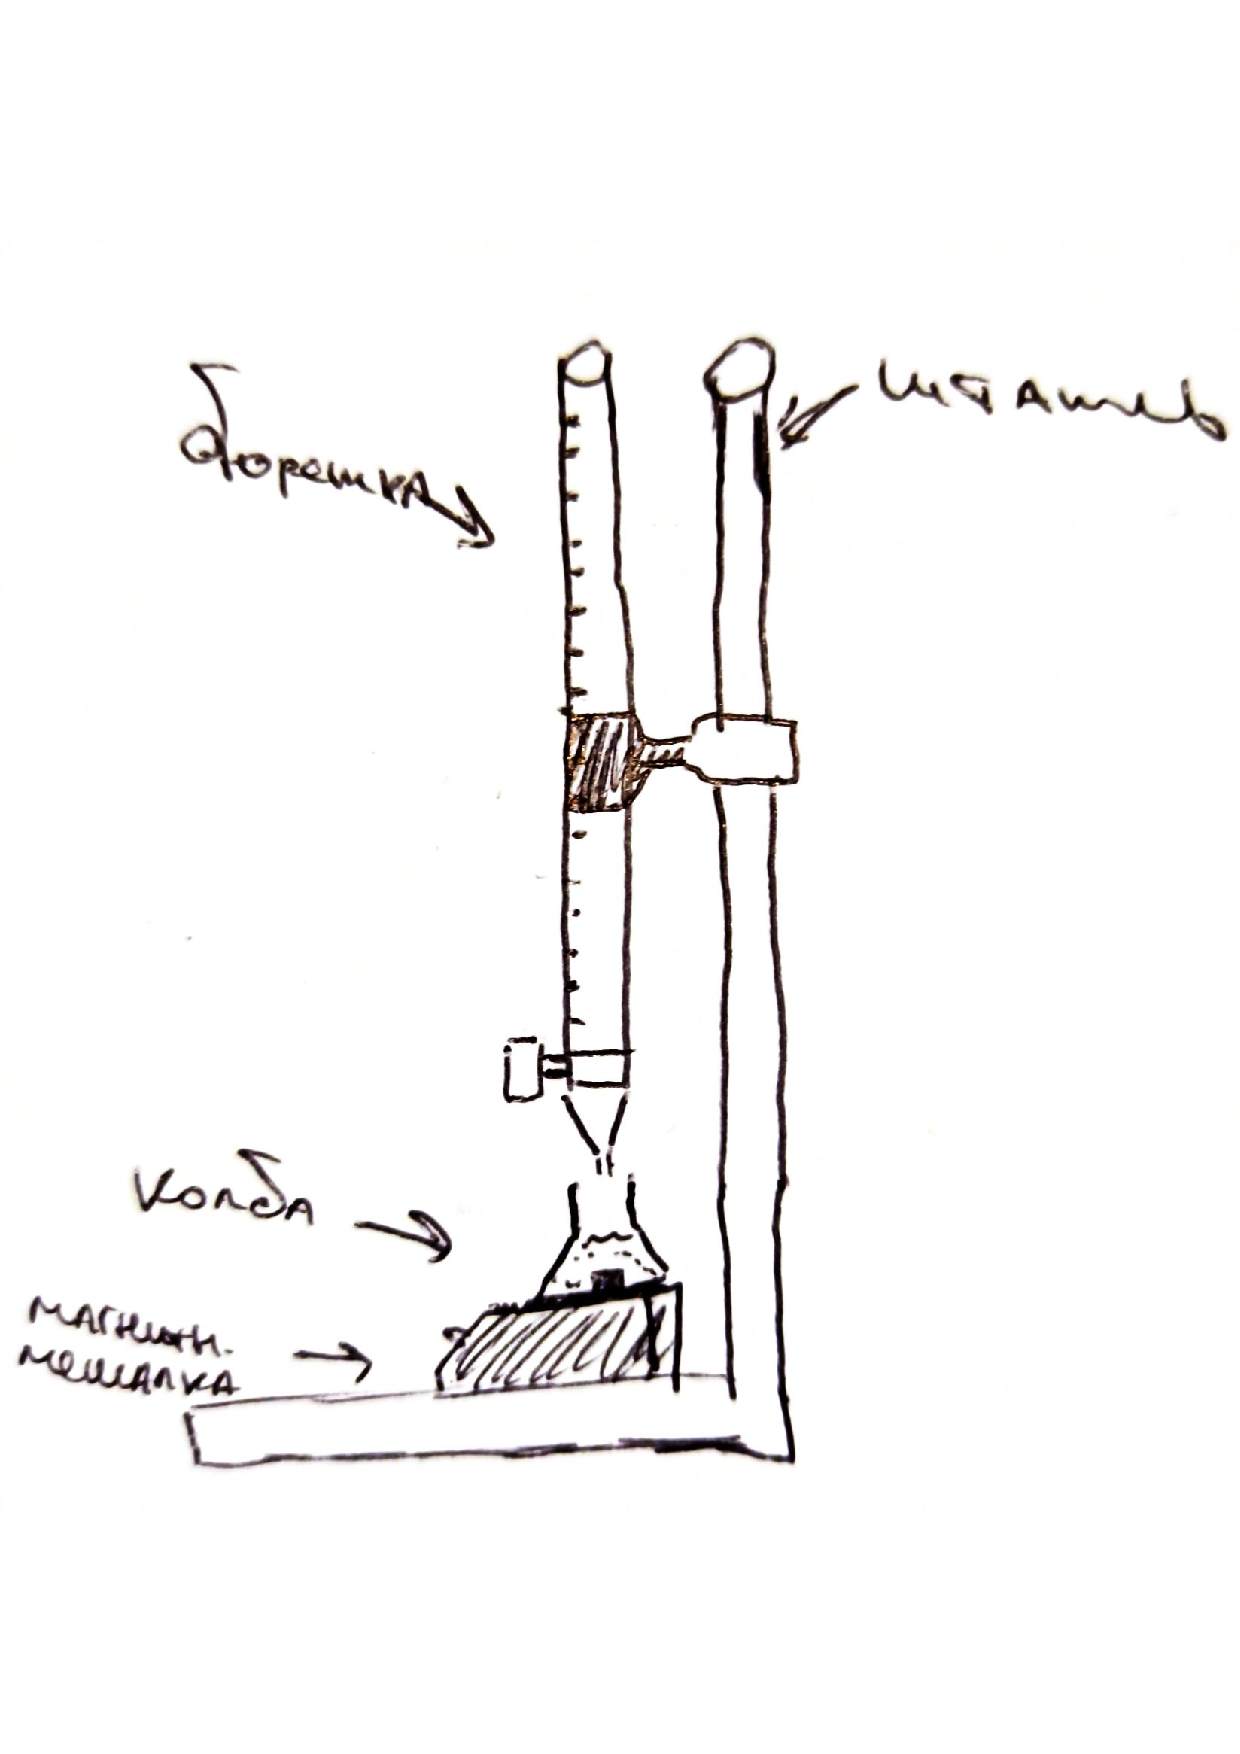
\includegraphics[width = 0.4\textwidth]{byuretka}
\end{center}

После этого в колбу с широким горлом было отмерено 10 мл 0.1 M раствора соляной кислоты, а также небольшой (2-3 капли) объем фенолфталеина. Затем, постоянно перемешивая раствор с помощью магнитной мешалки, в него постепенно, по капле, вносился раствор щелочи до получение устойчивой светло-розовой окраски. Необходимый для этого объем раствора щелочи был записан для последующей обработки. 

Последний этап был повторен 3 раза для получение более надежного результата.

\subsection{Полученные данные}

В результате серии экспериментов был получен следующий набор данных:

\begin{center}
	
	\begin{tabular}{|c|c|}
		\hline
		№ & Объем раствора NaOH, мл \\
		\hline
		1 & 12.5 \\
		\hline
		2 & 12 \\
		\hline
		3 & 11.8 \\
		\hline
	\end{tabular}
	
\end{center}

Таким образом, принимаем за необходимый объем среднее значение объема раствора и получаем $V_{nec} \approx 12.1$ мл.

\subsection{Обработка полученных результатов}

\subsubsection{Определение концентрации раствора щелочи}

При добавлении к соляной кислоте в колбе щелочи происходит реакция нейтрализации, которая описывается следующей формулой:

\begin{equation}
\ce{HCl + NaOH -> NaCl + H2O}
\label{eq:react}
\end{equation}

Рассчитаем количество вещества \ce{HCl} в исходном растворе соляной кислоты:

\begin{equation}
\nu_{HCl} = V C_{m HCl} = 0.01 \cdot 0.1 = 0.001 \text{ моль}
\end{equation}

Согласно уравнению реакции \ref{eq:react}, количество вещества \ce{NaOH} должно быть таким же, т.е.:

\begin{equation}
\nu_{NaOH} = \nu_{HCl} = 0.001 \text{ моль}
\end{equation}

Таким образом, реальная концентрация раствора, которую мы получаем с помощью метода титрования, оказывается равной:

\begin{equation}
\boxed{
	C_{mr} = \frac{\nu_{NaOH}}{V_{nec}} = \frac{0.001}{0.0121} \approx 0.08 \text{ М}
}
\end{equation}

В целом, полученная концентрация несколько отличается от той, которой мы пытались добиться.

\bigskip

\subsection{Выводы}

\begin{enumerate}
	\item Неточность в результатах может быть связана с тем, что неизвестно при каком pH индикатор меняет окраску (а в расчете предполагается что при pH = 7). Кроме того, погрешность может быть связана с неточностями c массой NaOH и своевременным прекращением подачи его раствора.
	
	\item Различие в результатах, возникающее при использовании разных индикаторов можно объяснить различием в значениях pH, при которых индикатор меняет свой цвет.
	
	\item Помимо указанных причин отличий эксперимента от ожидаемых теоретических результатов, возможным фактором отличия является также несовершенство метода хранения \ce{NaOH}, который на воздухе быстро поглощает водяной пар и углекислый газ, из-за чего мы получаем реактив с примесями.
\end{enumerate}

\section{Опыт 1.3: Гидролиз солей}

\subsection{Реактивы и оборудование}

\begin{itemize}
	\item Сухие соли: \ce{CH3COONa}, \ce{NaHCO3}, \ce{MnSO4}, \ce{Na2SO3}, \ce{NaCl},  \ce{Na2CO3}, \ce{ZnCl2}, \ce{NH4Cl}
	
	\item Спиртовка
	
	\item Пробирки
	
	\item Шпатель для реактивов
	
	\item Стеклянная палочка
\end{itemize}

\subsection{Порядок выполнения опыта}

В 8 пробирок были добавлены по одному микрошпателю указанных сухих солей, после чего они были разбавлены одинаковым небольшим количеством дистиллированной воды. Все растворы были тщательно перемешаны стеклянной палочкой. Затем показания pH снимались лакмусовой бумагой.

В результате были получены следующие значения для pH:


\begin{center}
\begin{tabular}{|c|c|c|c|c|c|c|c|c|}
	\hline
	В-во & \ce{CH3COONa} & \ce{NaHCO3} & \ce{MnSO4} & \ce{Na2SO3} & \ce{NaCl} & \ce{Na2CO3} & \ce{ZnCl2} & \ce{NH4Cl} \\
	\hline
	pH & 7-8 & 8-9 & 5-6 & 8-9 & 7 & 9-10 & 3-4 & 5-6 \\
	\hline
\end{tabular}
\end{center}

Соли, образованные сильным основанием и сильной кислотой не подвергаются гидролизу. Из исследованных солей не подвергается гидролизу только \ce{NaCl}.

\subsection{Уравнения реакций}

\begin{itemize}
	\item \ce{CH3COONa} --- гидролиз по аниону:
	
	\ce{CH3COO- + HOH <=> CH3COOH + OH-} 
	
	\ce{CH3COONa + HOH <=> CH3COOH + NaOH}
	
	\item \ce{NaHCO3} --- гидролиз по аниону:
	
	\ce{NaHCO3 + HOH <=> NaOH + H2CO3}
	
	\ce{HCO3- + HOH <=> OH- + H2CO3}
	
	\item \ce{2MnSO4} --- гидролиз по катиону:
	
	\textbf{1 ступень}
	
	\ce{2MnSO4 + 2HOH <=> (MnOH)2SO4 + H2SO4}
	
	\ce{Mn^2+ + HOH <=> MnOH^{-1} + H+}
	
	\textbf{2 ступень}
	
	\ce{(MnOH)2SO4 + 2HOH <=> Mn(OH)2 + H2SO4}
	
	\ce{MnOH+ + HOH <=> Mn(OH)2 + H+}.
	
	\item \ce{Na2SO3} --- гидролиз по аниону:
	
	\textbf{1 ступень}
	
	\ce{SO3^2- + HOH <=> HSO3- + OH-}
	
	\ce{Na2SO3 + HOH <=> NaHSO3 + NaOH}
	
	\textbf{2 ступень}
	
	\ce{HSO3- + HOH <=> H2SO3 + OH-}
	
	\ce{NaHSO3 + HOH <=> H2SO3 + NaOH}
	
	\item \ce{Na2CO3} --- гидролиз по аниону:
	
	\textbf{1 ступень}
	
	\ce{CO3^2- + HOH <=> HCO3- + OH-}
	
	\ce{Na2CO3 + HOH <=> NaHCO3 + NaOH}
	
	\textbf{2 ступень}
	
	\ce{HCO3- + HOH <=> H2CO3 + OH-}
	
	\ce{NaHCO3 + HOH <=> H2CO3 + NaOH}
	
	\item \ce{NaCl} --- гидролиз не идет.
	
	\item \ce{ZnCl2} --- гидролиз по катиону:
	
	\textbf{1 ступень}
	
	\ce{Zn^2+ + HOH <=> ZnOH+ + H+}
	
	\ce{ZnCl2 + HOH <=> ZnOHCl + HCl}
	
	\textbf{2 ступень}
	
	\ce{ZnOH+ + HOH <=> Zn(OH)2 + H+}
	
	\ce{ZnOHCl + HOH <=> Zn(OH)2 + HCl}
	
	\item \ce{NH4Cl} --- гидролиз по катиону:
	
	\ce{NH4Cl + HOH <=> NH4OH + HCl}
	
	\ce{NH4+- + HOH <=> ONH4OH + H+}
	
\end{itemize}

Отличие pH растворов карбоната и гидрокарбоната натрия объясняется тем, что у карбоната натрия гидролиз идет в 2 ступени, в то время как у гидрокарбоната натрия в одну

\subsection{Влияние температуры на степень гидролиза}
\begin{center}
	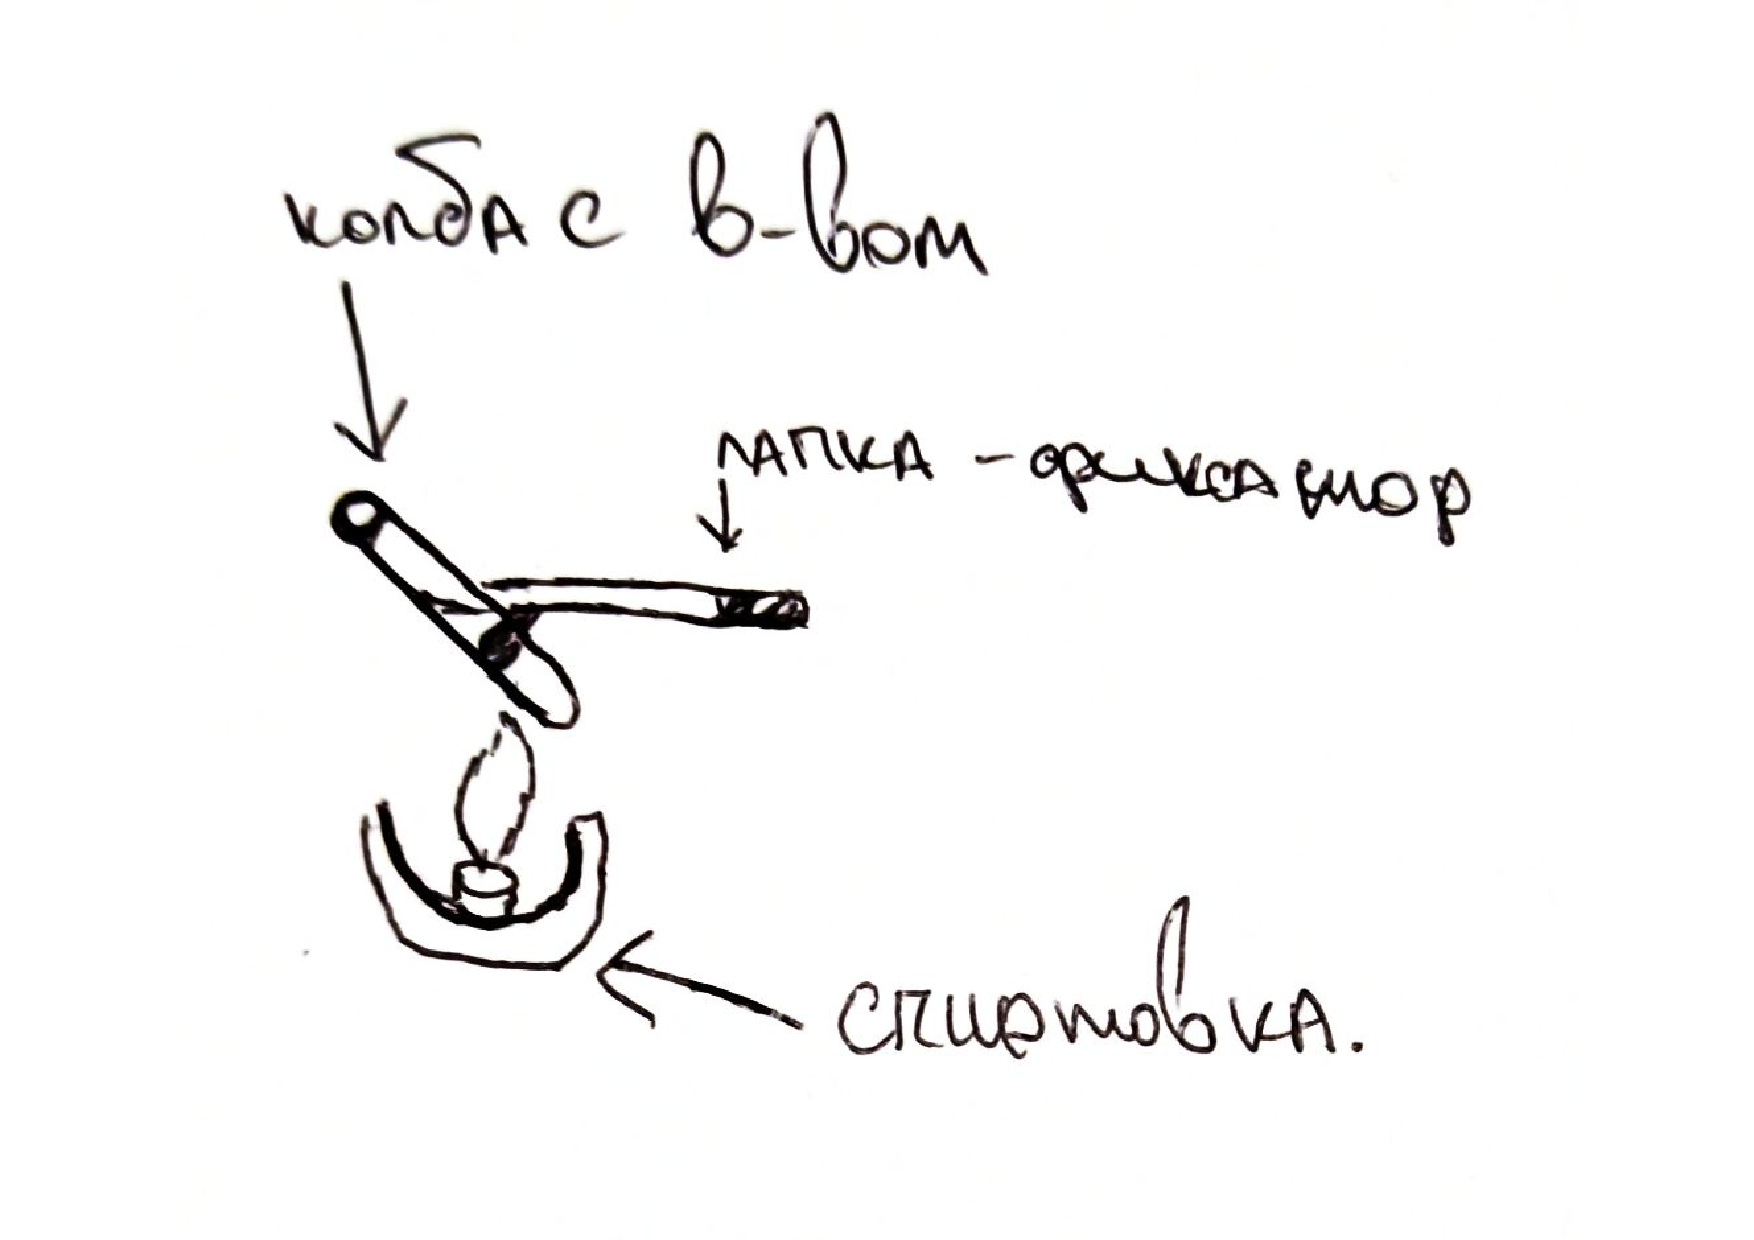
\includegraphics[width = 0.4\textwidth]{Nagrev}\\
\end{center}

\begin{itemize}
	\item При добавлении фенолфталеина раствор ацетата натрия остался бесцветным 
	\item При нагревании раствор становился все более розовым
	\item При охлаждении раствор вновь обесцвечивался
\end{itemize}

Изменение окраски говорит об изменении pH раствора при температурном воздействии.

\subsection{Выводы}
pH раствора может зависить от:
\begin{itemize}
	\item температуры раствора 
	\item компонентов соли
	\item количества ступеней в процессе гидролиза
\end{itemize}

\section{Опыт 1.4: Гидрокомплексы металлов и их свойства}

\subsection{Реактивы и оборудование}

\begin{itemize}
	\item Растворы: \ce{ZnCl2}, \ce{CuSO4}, \ce{MnCl2}, \ce{NaOH}
	
	\item Пробирки
\end{itemize}

\subsection{Порядок выполнения}

В пробирки были внесены растворы солей. Далее, для исследования осадка добавлялось несколько капель щелочи. Затем, было исследовано растворение осадка в избытке щелочи

Было получено, что во всех заданных растворах при добавлении раствора NaOH выпадает осадок. Кроме того, в растворе \ce{ZnCl2} осадок растворился в избытке щелочи.

\subsection{Уравнения реакций:}

\begin{itemize}
	\item \ce{ZnCl2}:
	
	\ce{ZnCl2 + 2NaOH <=> 2NaCl + Zn(OH)2 v}
	
	\ce{ZnCl2 + 4NaOH <=> 2NaCl + Na2(OH)2} - тетрагидроксоцинкат(II) натрия
	
	\item \ce{CuSO4}:
	
	\ce{CuSO4 + 2NaOH <=> Na2SO4 + Cu(OH)2}
	
	\ce{CuSO4 + 4NaOH <=> Na2SO4 + Na2[Cu(OH)4] v} - тетрагидроксокупрат(II) натрия
	
	\item \ce{MnCl2}:
	
	\ce{MnCl2 + 2NaOH <=> 2NaCl + Mn(OH)2 v}
	
	\ce{Zn(OH)2} --- Амфотерный гидроксид
	\ce{Cu(OH)2} --- Основный гидроксид
	\ce{Mn(OH)2} --- Основный гидроксид
	
\end{itemize}

\end{document}